
\chapter{$\beta$-Ensembles}

%%%%%%%%%%%%%%%%%%%%%%%%%%%%%%%%%%%%%%%%%%%%%%%%%%%%%%%%%%%%%%%%%%%%%%%%%%%%%%%%%%%%%%%%%%
%%%%%%%%%%%%%%%%%%%%%%%%%%%%%%%%%%%%%%%%%%%%%%%%%%%%%%%%%%%%%%%%%%%%%%%%%%%%%%%%%%%%%%%%%%
\section{Introduction}
So, what are \textit{eigenvalue dispersions}? 

\begin{figure}[h]
	% the options are h = here, t = top, b = bottom, p = page of figures.
	% you can add an exclamation mark to make it try harder, and multiple
	% options if you have an order of preference, e.g.
	% \begin{figure}[h!tbp]
	   
	       \centering
	    % DO NOT ADD A FILENAME EXTENSION TO THE GRAPHIC FILE
	    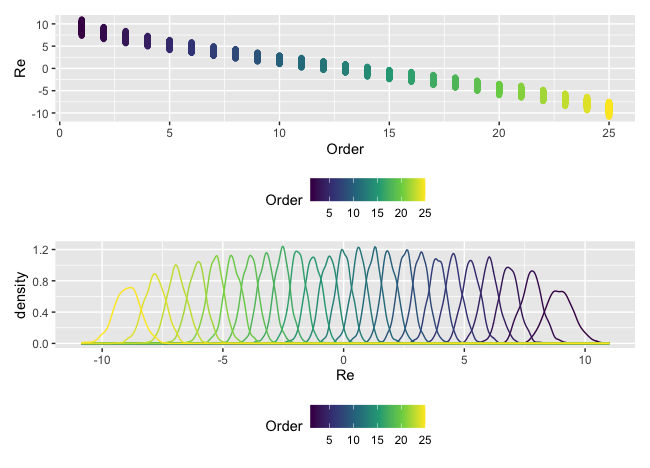
\includegraphics[scale = 0.6]{chapters/graphics/c2_order_sign}
	     \caption{A Figure}
	 \label{subd}
	\end{figure}


%%%%%%%%%%%%%%%%%%%%%%%%%%%%%%%%%%%%%%%%%%%%%%%%%%%%%%%%%%%%%%%%%%%%%%%%%%%%%%%%%%%%%%%%%%

\section{Section I}


